%% LaTeX Beamer presentation template (requires beamer package)
%% see http://bitbucket.org/rivanvx/beamer/wiki/Home
%% idea contributed by H. Turgut Uyar
%% template based on a template by Till Tantau
%% this template is still evolving - it might differ in future releases!

\documentclass{beamer}

\mode<presentation>
{
\usetheme{CIn20131120}

%\setbeamercovered{transparent}
}

\usepackage[english]{babel}
\usepackage[utf8]{inputenc}
\usepackage[T1]{fontenc} 

% font definitions, try \usepackage{ae} instead of the following
% three lines if you don't like this look
\usepackage{mathptmx}
\usepackage[scaled=.90]{helvet}
\usepackage{courier}
\usepackage{tikz}
\usepackage{varwidth}
\usepackage{xspace}
\usepackage{verbatim}
\usepackage{environ}
\usepackage{ifthen}

\usetikzlibrary{arrows,trees,positioning,circuits.logic.US,shapes}

\DeclareGraphicsExtensions{.png,.eps}
%\DeclareGraphicsExtensions{.png}
\graphicspath{{./images/},{./}}


\usepackage[T1]{fontenc}

\DeclareMathOperator{\doo}{d}
\DeclareMathOperator{\nibefore}{\lhd}
\DeclareMathOperator{\simultaneous}{\triangle}
\DeclareMathOperator{\ibefore}{\unlhd}
\DeclareMathOperator{\inter}{\cap}
\DeclareMathOperator{\union}{\cup}
\DeclareMathOperator{\tvar}{\mathsf{tvar}}
\DeclareMathOperator{\distinct}{\mathsf{distinct}}
\DeclareMathOperator{\set}{\mathsf{set}}
\DeclareMathOperator{\xbefore}{\rightarrow}
\DeclareMathOperator{\listt}{\mathsf{list}}
\DeclareMathOperator{\sett}{\mathsf{set}}
\DeclareMathOperator{\tformulat}{\mathsf{tformula}}
\DeclareMathOperator{\BasicEventMinLevel}{\mathsf{BasicEventMinLevel}}
\DeclareMathOperator{\RootProbability}{\mathsf{RootProbability}}
\DeclareMathOperator{\evaluateRule}{\mathsf{evaluateRule}}
\DeclareMathOperator{\minBasicEventLevel}{\mathsf{minBasicEventLevel}}
\DeclareMathOperator{\ftProbability}{\mathsf{ftProbability}}
\DeclareMathOperator{\defs}{\doteq}
\DeclareMathOperator{\concat}{@}
%\newcommand{\aaexp}[2]{^{#1}/_{#2}}
\newcommand{\aaexp}[2]{{\left[#1\right]}^{\left[#2\right]}}
\newcommand{\nominalvalue}[2]{\mathsf{N}^{#2}\left(#1\right)}
\newcommand{\failurevalue}[2]{\mathsf{#1}^{#2}}
\newcommand{\component}[1]{\mathsf{C}^{#1}}
\newcommand{\outvalue}[2]{\mathsf{#1}^{#2}}
\newcommand{\outvalueof}[1]{\rho\left(#1\right)}
\def\fba{fba}
\def\tfa{tfa}

\newcommand{\includeautosizegraphics}[1]{%
\includegraphics[height=0.8\textheight,width=\textwidth,keepaspectratio]{#1}%
}

\def\tikzoverlay{%
   \tikz[baseline,overlay]\node[every overlay node]
}

\tikzstyle{every overlay node}=[draw=black,fill=white,rounded corners,anchor=north west]

\tikzstyle{event text}=[text centered, 
  execute at begin node={\begin{varwidth}{2cm}},
  execute at end node={\end{varwidth}}
  ]
  
\tikzstyle{event}=[event text, rectangle, draw=black, fill=yellow!20, anchor=north]
%\tikzstyle{fault tree}=[edge from parent fork down, sibling distance=7cm, level distance=1.4cm, circuit logic US, growth parent anchor=south,nodes=event]
\tikzstyle{fault tree}=[circuit logic US]

\tikzstyle{level 1}=[sibling distance=7cm, level distance=1.4cm, growth parent anchor=south, nodes=event]
\tikzstyle{level 2}=[sibling distance=5cm]
\tikzstyle{level 3}=[sibling distance=5cm]
\tikzstyle{level 4}=[sibling distance=3cm]

\tikzstyle{gate}=[rotate=90, anchor=east, xshift=-1mm]
\tikzstyle{or gate}=[gate, or gate US,fill=blue!60]
\tikzstyle{and gate}=[gate, and gate US, fill=red!60]
\tikzstyle{basic}=[circle, fill=green!60, anchor=north, minimum width=0.5cm]

\tikzstyle{spare gate}=[shape=spare gate, fill=orange!40]
  
\tikzset{
  >=stealth',
  edge from parent path={(\tikzparentnode.south) -- ++(0,-0.95cm)
      -| (\tikzchildnode.north)},
  global scale/.style={
    scale=#1,
    every node/.style={scale=#1}
  }
}
\makeatletter
\pgfdeclareshape{spare gate}{
  \inheritsavedanchors[from=circle]
  \inheritanchor[from=circle]{center}
  \inheritanchor[from=circle]{north}
  \inheritanchor[from=circle]{south}
  \inheritanchor[from=circle]{east}
  \inheritanchor[from=circle]{west}
  \backgroundpath{%
      % Save radius to x
      \pgf@x=\radius
      % Radius is also containing the "minimum width" and "minimum height"
      % This ensures that even with no text the shape will be drawn.
      % Unless of course that min are set to 0pt
      % So no need to check for that
      % Save radius
      \pgfutil@tempdima=\pgf@x%

      % west triangle corner "b"
      \pgf@xb=-3\pgf@x%
      \pgf@yb=-4\pgf@x%
      % east triangle corner "c"
      \pgf@xc= 3\pgf@x%
      \pgf@yc=-4\pgf@x%

      % If text is present shift shape to center 
      % You need to shift more, but to get the idea
      \centerpoint
      \advance\pgf@xb by\pgf@x
      \advance\pgf@yb by\pgf@y
      \advance\pgf@xc by\pgf@x
      \advance\pgf@yc by\pgf@y

      % Save centerpoint in "a" (top triangle point)
      \pgf@xa=\pgf@x 
      \pgf@ya=\pgf@y

      % Below are good for debugging purposes.
      %\message{^^JTop : \the\pgf@xa,\the\pgf@ya}
      %\message{^^JWest: \the\pgf@xb,\the\pgf@yb}
      %\message{^^JEast: \the\pgf@xc,\the\pgf@yc}
      %\message{^^JCent: \the\pgf@x,\the\pgf@y}

      % draw triangle..
      \pgfpathmoveto{\pgfpoint{\pgf@xa}{\pgf@ya}}%
      \pgfpathlineto{\pgfpoint{\pgf@xb}{\pgf@yb}}%
      \pgfpathlineto{\pgfpoint{\pgf@xc}{\pgf@yc}}%
      \pgfpathclose

      % The radius of the small circles
      % Read in from option TODO
      \pgfutil@tempdimb=3pt

      % Move top triangle to head circle
      \advance\pgf@ya by.25\pgfutil@tempdimb
      % Move west triangle corner to west circle center
      \advance\pgf@xb by 1.5\pgfutil@tempdima
      \advance\pgf@yb by -\pgfutil@tempdimb
      % For handling line thickness if you wish "edge touch" and not "overlap"
      %\advance\pgf@yb by -.5\pgflinewidth 
      % Move east triangle corner to east circle center
      \advance\pgf@xc by-1.5\pgfutil@tempdima
      \advance\pgf@yc by -\pgfutil@tempdimb
      % For handling line thickness if you wish "edge touch" and not "overlap"
      %\advance\pgf@yc by -.5\pgflinewidth

      % This saves underlying "stuff" when you have the explicit `\pgfqpoint` and is thus a little faster
      \edef\pgf@marshal{%
          \noexpand\pgfpathcircle{%
              \noexpand\pgfqpoint{\the\pgf@xa}{\the\pgf@ya}}
          {\the\pgfutil@tempdimb}%
          \noexpand\pgfpathcircle{%
              \noexpand\pgfqpoint{\the\pgf@xb}{\the\pgf@yb}}
          {\the\pgfutil@tempdimb}%
          \noexpand\pgfpathcircle{%
              \noexpand\pgfqpoint{\the\pgf@xc}{\the\pgf@yc}}
          {\the\pgfutil@tempdimb}%
      }\pgf@marshal
  }
}
\makeatother

\def\CSPM{CSP$_M$\xspace}


\newenvironment{snippetcspm}[1][2]
{
\ifthenelse{\equal{#1}{0}}
    {\tiny}
    {
    \ifthenelse{\equal{#1}{1}}
        {\scriptsize}
        {
        \ifthenelse{\equal{#1}{2}}
            {\footnotesize}
            {\small}
        }
    }
%\begin{samepage}
\verbatim
}
{
\endverbatim
%\end{samepage}
}




\title{Fault Tree Analysis with Temporal Faults Algebra}
\subtitle{A formal approach to verify safety requirements}

%\subtitle{}

% - Use the \inst{?} command only if the authors have different
%   affiliation.
%\author{F.~Author\inst{1} \and S.~Another\inst{2}}
\author{André Didier}

% - Use the \inst command only if there are several affiliations.
% - Keep it simple, no one is interested in your street address.


\date{11 May 2015}


% This is only inserted into the PDF information catalog. Can be left
% out.
\subject{Talks}



% If you have a file called "university-logo-filename.xxx", where xxx
% is a graphic format that can be processed by latex or pdflatex,
% resp., then you can add a logo as follows:

% \pgfdeclareimage[height=0.5cm]{university-logo}{university-logo-filename}
% \logo{\pgfuseimage{university-logo}}



% Delete this, if you do not want the table of contents to pop up at
% the beginning of each subsection:
% \AtBeginSubsection[]
% {
% \begin{frame}<beamer>
% \frametitle{Outline}
% \tableofcontents[currentsection,currentsubsection]
% \end{frame}
% }

% If you wish to uncover everything in a step-wise fashion, uncomment
% the following command:

%\beamerdefaultoverlayspecification{<+->}

\begin{document}

\begin{frame}
\titlepage
\end{frame}

\begin{frame}
\frametitle{A safety problem\ldots}
\begin{enumerate}
  \item Analyse \alert<4>{large} Dynamic Fault Trees (DFT)\\
    \begin{minipage}[c]{4.60cm}
        \begin{itemize}
          \item Static Fault Tree (SFT) 
          \item Temporal Fault Trees (TFT)
          \item DFT analysis 
        \end{itemize}
    \end{minipage}
    \begin{minipage}[c]{5.3cm}
    \only<2->{$\implies$ Does the system meet safety requirements?}
    \end{minipage}
  \item Formalise DFT qualitative and quantitative analysis
    \begin{itemize}
      \item<3-> Is the analysis reliable?
      \item<3-> Does the tree represent the system model?
    \end{itemize}
\end{enumerate}
\end{frame}

\begin{frame}
\frametitle{Concepts in this presentation}

\begin{itemize}
  \item \alert<2>{Systems modelling with Simulink}
  \item \alert<2>{Faults injection}
  \item \alert<2>{Faults traces}
  \item Fault Trees -- \alert<2>{Static}, Temporal and Dynamic
  \item Free Boolean Algebra
  \item Lists lattice
  \item Temporal Faults Algebra
  \item Activation Algebra and Predicates
  \item Safety requirements and fault tree acceptance criteria
\end{itemize}

\onslide<2>{\tikzoverlay[text width=1.8cm] at (5cm,5cm) {Master dissertation};}
\end{frame}

\section{Master dissertation review}

\begin{frame}
\frametitle{System modelling with Simulink}
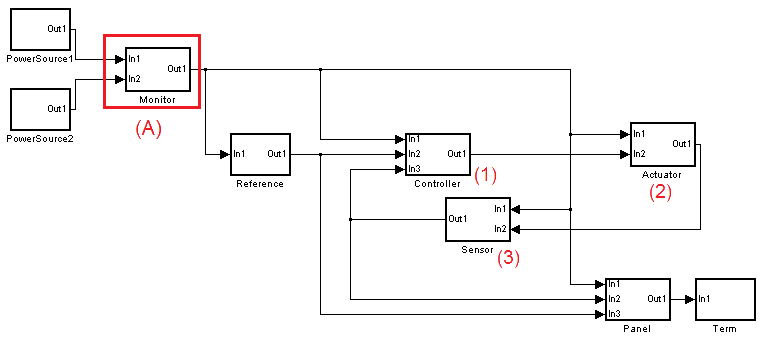
\includegraphics[width=\linewidth]{acsBlockDiagrams}
\end{frame}

\begin{frame}
\frametitle{Fault Tolerance, Failure Logic, Safety Analysis}
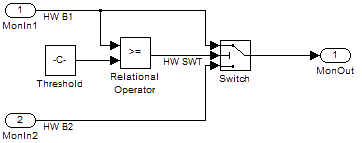
\includegraphics[height=0.4\textheight]{blockDiagramMonitorInternals}\par
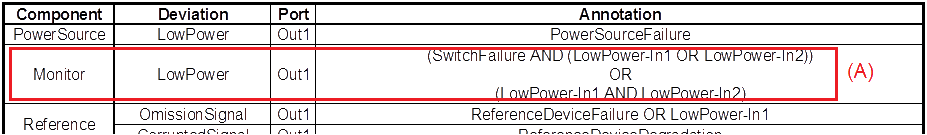
\includegraphics[width=\linewidth]{acsAnnotations}
\end{frame}

\begin{frame}[fragile]
\frametitle{\CSPM to inject faults and obtain fault traces}
From:\\
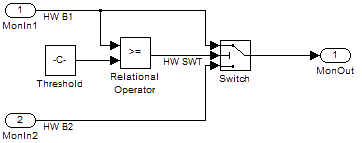
\includegraphics[height=0.3\textheight]{blockDiagramMonitorInternals}\par

We obtain traces with faults:
{\tiny
\begin{itemize}
  \item \verb|failure.Hardware.N04_RelationalOperator| -- HW SWT \onslide<2->{(S)}
  \item \verb|failure.Hardware.N04_MonIn1| -- HW B1 \onslide<2->{(A)}
  \item \verb|failure.Hardware.N04_MonIn2| -- HW B2 \onslide<2->{(B)}
\end{itemize}
}

\end{frame}

\begin{frame}[fragile]
\frametitle{Faults trace example}
Two of the 64 traces are:
\begin{snippetcspm}[0]
TRACE 1:
failure.Hardware.N04_MonIn2.1.EXP.I.5
failure.Hardware.N04_MonIn2.1.ACT.OMISSION
failure.Hardware.N04_RelationalOperator.1.EXP.B.true
failure.Hardware.N04_RelationalOperator.1.ACT.B.false
out.1.OMISSION

TRACE 2:
failure.Hardware.N04_MonIn1.1.EXP.I.5
failure.Hardware.N04_MonIn1.1.ACT.OMISSION
failure.Hardware.N04_MonIn2.1.EXP.I.5
failure.Hardware.N04_MonIn2.1.ACT.OMISSION
out.1.OMISSION
\end{snippetcspm}
\footnotesize
\begin{itemize}
  \item Combine each trace with conjunctions: $B \land S$, $A \land B$, \ldots
  \item Combine all traces with disjunctions: $(B \land S) \lor (A \land B) \lor \ldots$
  \item The complete failure logic after simplification is exactly the supplied by Embraer: \alert<4>{$(A \land B) \lor (S \land (A \lor B))$}
  \item <2-> Note that we ignore events order in each trace, because Boolean AND is commutative.
  \item<3-> Some traces appear in a specific order: $A$ then $S$, but not $S$ then $A$.
\end{itemize}

\onslide<4>{\tikzoverlay[text width=3cm] at (3.8cm,2.7cm) {a.k.a structure function or structure expression};}
\end{frame}

\section{Fault Trees}

\subsection{Static Fault Trees}

\begin{frame}
\frametitle{Static Fault Trees}
\begin{tikzpicture}[fault tree, global scale=0.7]
\node (r) [event] {Low Power}
    child {
      node (both) [event] {Both inputs fail}
      child { node (a1) [event] {A fails} } 
      child { node (b1) [event] {B fails} }
    }
    child {
      node (si) [event] {One input fails and the switcher fails}
      child { node (s) [event] {Switcher fails}}
      child { 
        node (oneinput) [event] {One input fails}
        child { node (a2) [event] {A fails} }
        child { node (b2) [event] {B fails} }
      }
    };

\node [or gate] (or1) at (r.south) {};
\node [and gate] (and1) at (both.south) {};
\node [and gate] at (si.south) {};
\node [or gate] at (oneinput.south) {};
\node [basic] at (a1.south) {};
\node [basic] at (a2.south) {};
\node [basic] at (b1.south) {};
\node [basic] at (b2.south) {};

\onslide<2->{
\node (rdescr) [above right=0.5cm and 0cm of r] {Root event};
\draw (rdescr) edge[->] (r);

\node (interdescr) [above right=0.5cm and 0cm of si] {Intermediary event};
\draw (interdescr) edge[->] (si);

\node (ordescr) [below right=0 and 0.5cm of or1] {OR gate};
\draw (ordescr) edge[->] (or1);

\node (anddescr) [below right=0 and 0.5cm of and1] {AND gate};
\draw (anddescr) edge[->] (and1);

\node (basicdescr) [below right=0.3 and 0.5cm of a1] {Basic event};
\draw (basicdescr) edge[->] (a1);
}

      %child {
      %  node [and gate] {}
      %  child {
      %    node [event] {One input fails and the switcher fails}
      %    child { node [basic] {Switcher fails} }
      %    child {
      %      node [event] {One input fails}
      %      child {
      %        node [or gate] {}
      %        child [basic] {A fails}
      %        child [basic] {B fails}
      %      }
      %    }
      %  }
      %}
\end{tikzpicture}
\end{frame}

\subsection{Dynamic Fault Trees}

\begin{frame}
\frametitle{Dynamic Fault Trees}
\begin{itemize}
  \item Priority AND -- PAND\\
    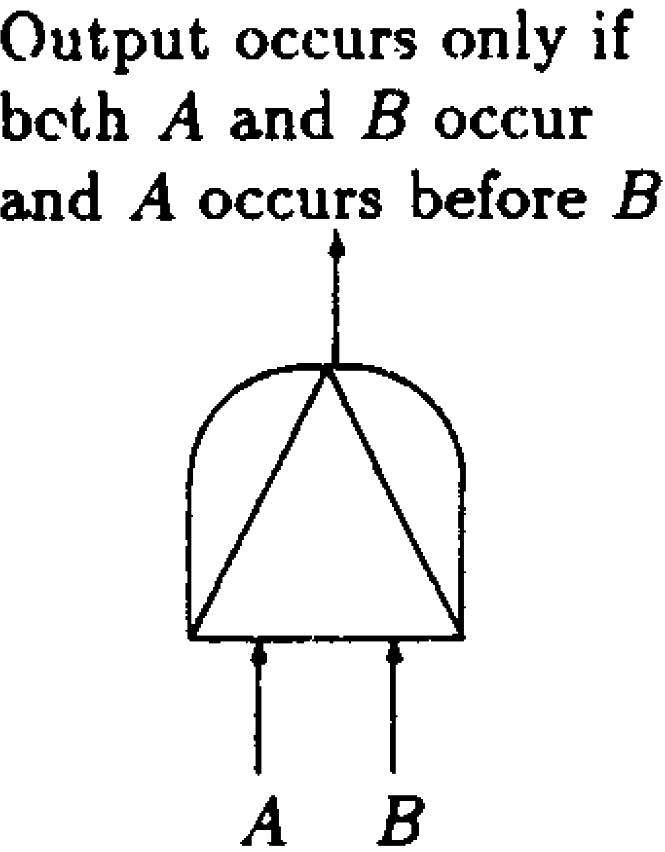
\includegraphics[height=4cm]{pand-dugan}
\end{itemize}
\end{frame}

\begin{frame}
\frametitle{Dynamic Fault Trees}
\begin{itemize}
  \item Cold Spare gate -- CSP\\
    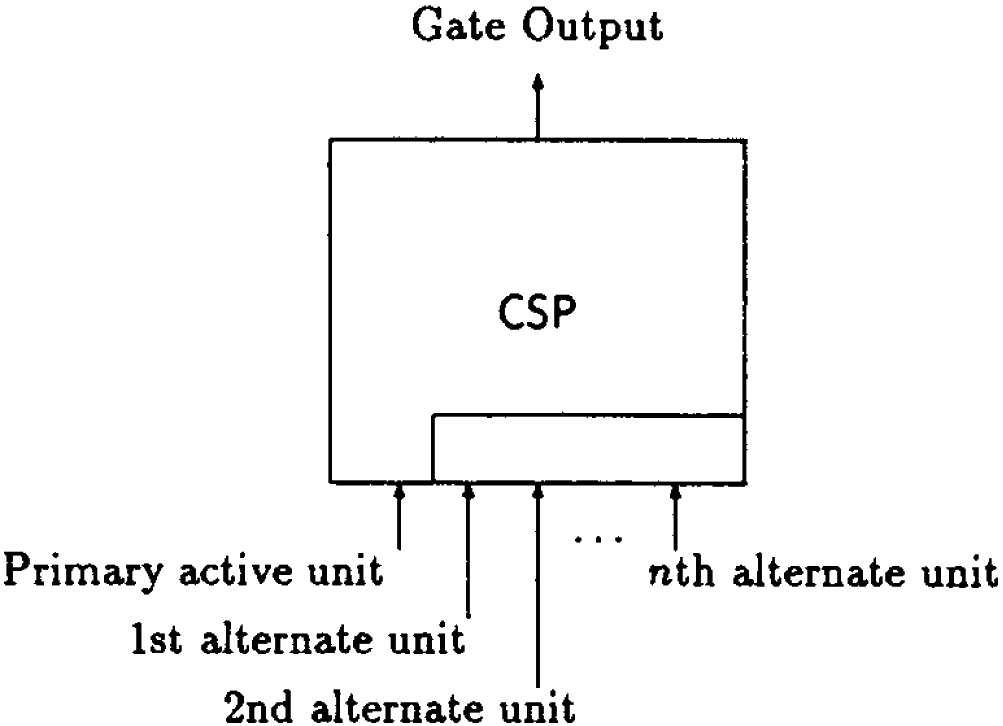
\includegraphics[height=4cm]{csp-dugan}
  \item Example: 4 tires, 1 spare
\end{itemize}
\end{frame}

\begin{frame}
\frametitle{Dynamic Fault Trees}
\begin{itemize}
  \item Sequence Enforcing gate -- SEQ (dummy output)\\
    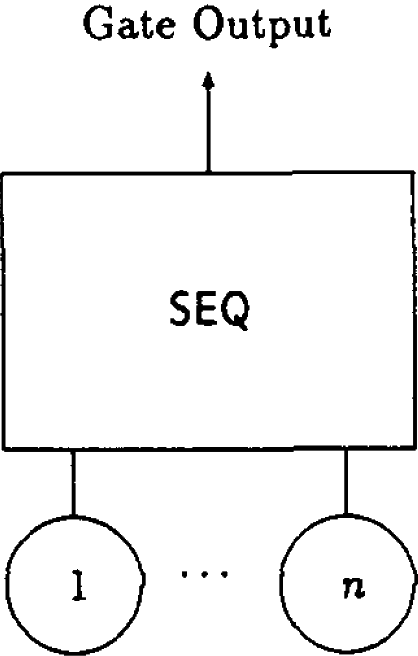
\includegraphics[height=4cm]{seq-dugan} 
  \item Events are forced to occur in a specific order
\end{itemize}
\end{frame}

\begin{frame}
\frametitle{Dynamic Fault Trees}
\begin{itemize}
  \item Functional Dependency gate -- FDEP (dummy output)\\
    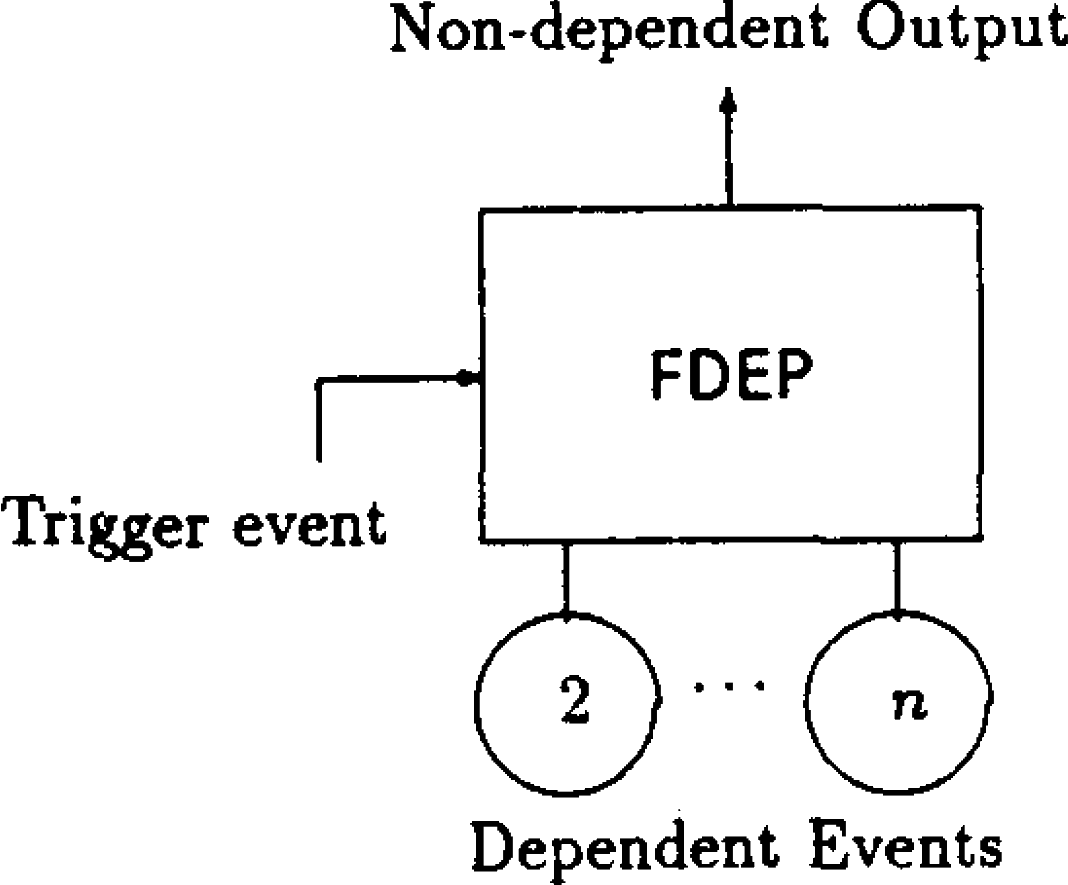
\includegraphics[height=4cm]{fdep-dugan}
  \item Dependent events are forced to occur when the trigger events activates;
  \item Otherwise they are independent.
\end{itemize}
\end{frame}

\begin{frame}
\frametitle{Relevant DFT gates}
\begin{itemize}
  \item SEQ is expressible in terms of CSP.
  \item For DFT, the relevant gates are then PAND, FDEP and CSP. 
\end{itemize}
\end{frame}

\subsection{Temporal Fault Trees}

\begin{frame}
\frametitle{Temporal Fault Trees}
\begin{itemize}
  \item Priority AND gate -- PAND\\
  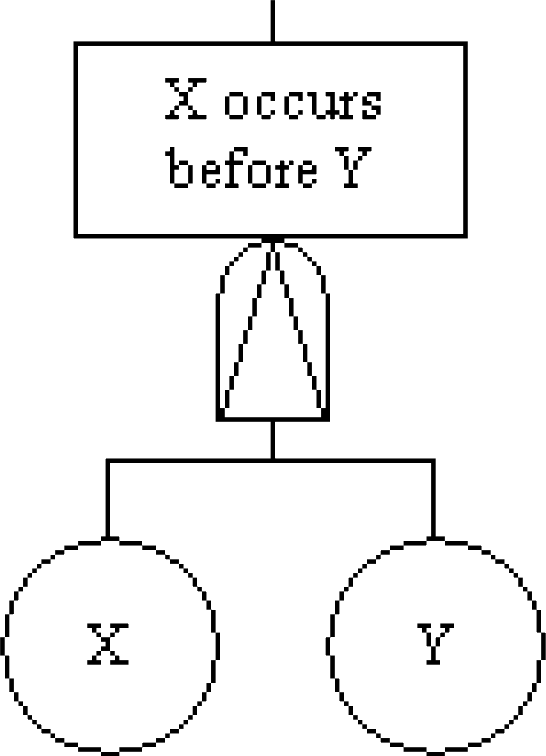
\includegraphics[height=4cm]{pand-walker}
\end{itemize}
\end{frame}

\begin{frame}
\frametitle{Temporal Fault Trees}
\begin{itemize}
  \item Priority OR gate -- POR\\
  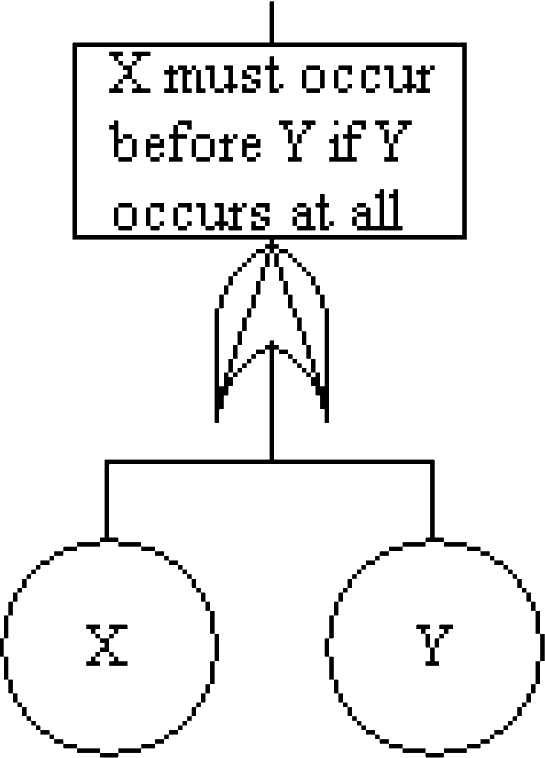
\includegraphics[height=4cm]{por-walker}
\end{itemize}
\end{frame}

\begin{frame}
\frametitle{Temporal Fault Trees}
\begin{itemize}
  \item Simultaneous gate -- SAND\\
  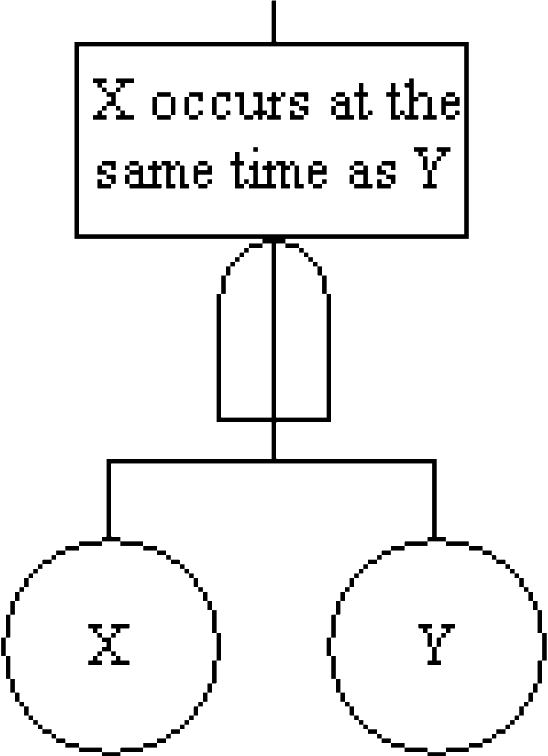
\includegraphics[height=4cm]{sand-walker}
\end{itemize}
\end{frame}



\end{document}
